\documentclass[12pt,a4paper]{article}
\usepackage[T5]{fontenc}
\usepackage{graphicx}
\usepackage[hidelinks]{hyperref}
\usepackage{float}
\usepackage{indentfirst}
\title{\textbf{BÁO CÁO THỰC HÀNH BUỔI 3}}
\author{\textbf{Tuấn Dũng Nguyễn, ID: 24020456}}
\date{}
\begin{document}
	\maketitle
	\section*{Bài 1}
	\begin{figure}[H]
		\centering
		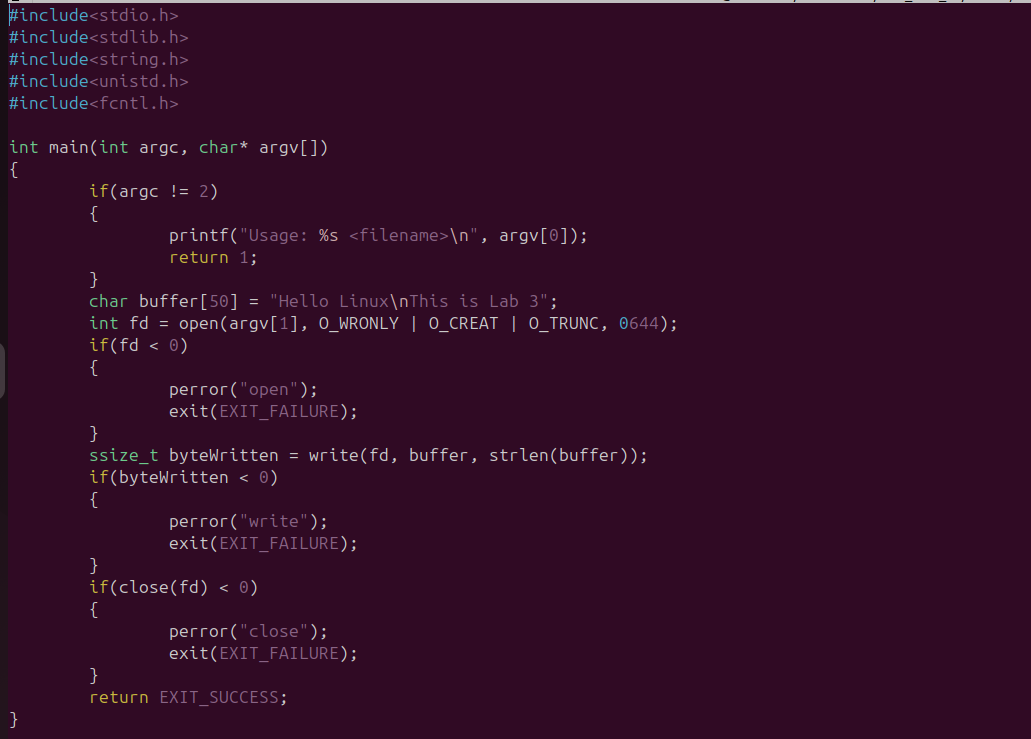
\includegraphics[width=0.7\linewidth]{figures/e1}
		\caption{Mã nguồn chương trình createfile.}
		\label{fig:e1}
	\end{figure}
	
	Tương tự ở bài trên, em cũng truyền 2 tham số vào hàm \texttt{main}. Để mở và tạo file \texttt{filename} em dùng hàm \texttt{open()} với các flags: \texttt{O\_WRONLY} để ghi nội dung vào file, \texttt{O\_CREAT, O\_TRUNC} để tạo file và xóa toàn bộ nội dung trong file (nếu đã tồn tại), cấp quyền đọc và ghi cho owner bằng mã 0644 (tương đương với lệnh \texttt{chmod 0644 filename}).
	
	Kết quả khi chạy kiểm tra chương trình:
	\begin{figure}[H]
		\centering
		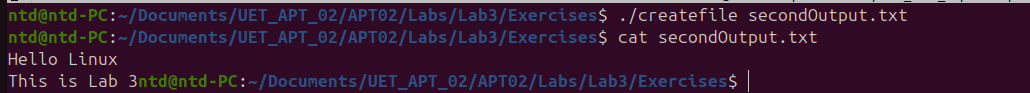
\includegraphics[width=0.7\linewidth]{figures/e1_result_1}
		\caption{Kết quả chạy chương trình createfile với secondOutput.txt}
		\label{fig:e1result1}
	\end{figure}
	
	\section*{Bài 2}
	\begin{figure}[H]
		\centering
		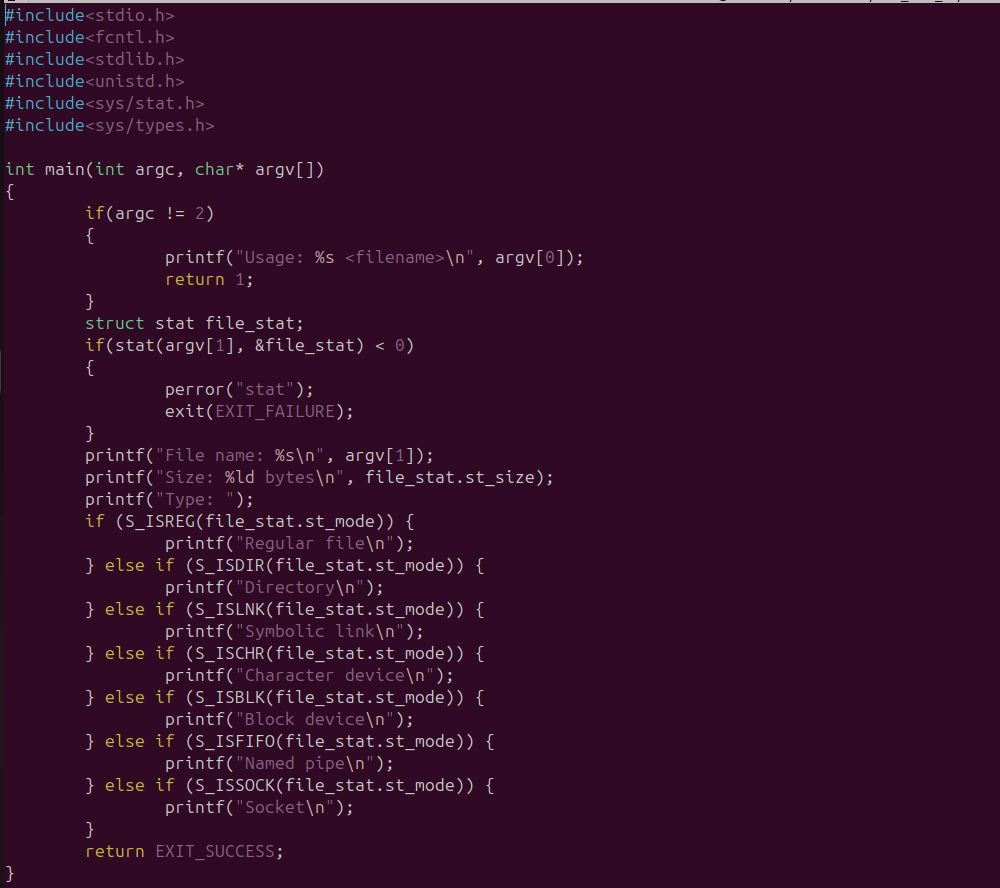
\includegraphics[width=0.7\linewidth]{figures/e2}
		\caption{Mã nguồn chương trình fileinfo.}
		\label{fig:e2}
	\end{figure}
	
	Khi khai báo hàm main, em khai báo thêm 2 tham số \texttt{int argc} và \texttt{char* argv[]}để khi chạy chương trình, hàm main nhận trực tiếp tham số (là tên của file cần xem info) liền sau lệnh chạy chương trình \texttt{./fileinfo}.
	
	Tham số \texttt{argc} sẽ đếm và lưu trữ số lượng đối số khi thực thi chương trình (đếm cả lệnh gọi chương trình), ở đây em kiểm tra là 2 đối số trong lệnh \texttt{./fileinfo filename.txt} có tổng là 2 đối số.
	
	Tham số \texttt{char *argv[]} sẽ lưu trữ lại chuỗi ký tự được nhập vào ngay sau khi chạy chương trình qua lệnh \texttt{./fileinfo filename.txt} (chính là chuỗi \texttt{filename.txt}).
	
	
	Cấu trúc \texttt{struct stat} được định nghĩa trong thư viện \texttt{sys/wait}, em khai báo biến \texttt{file\_stat} thuộc kiểu cấu trúc này để kiểm tra thông tin của \texttt{filename.txt}.
	
	Kết quả khi chạy kiểm tra chương trình trong hình \ref{fig:e2result}
	\begin{figure}[H]
		\centering
		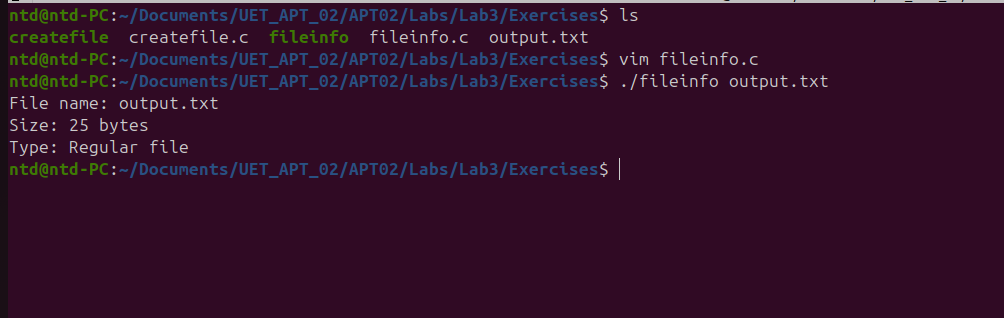
\includegraphics[width=0.7\linewidth]{figures/e2_result}
		\caption{Kết quả khi chạy trên file output.txt.}
		\label{fig:e2result}
	\end{figure}
	Để xác định loại của file này em truy cập đến thuộc tính \texttt{file\_stat.st\_mode} và dùng bảng các kết quả có thể của tính \texttt{st\_mode} để lọc ra các loại fiBài
	
	\section*{Bài 3}
	\begin{figure}[H]
		\centering
		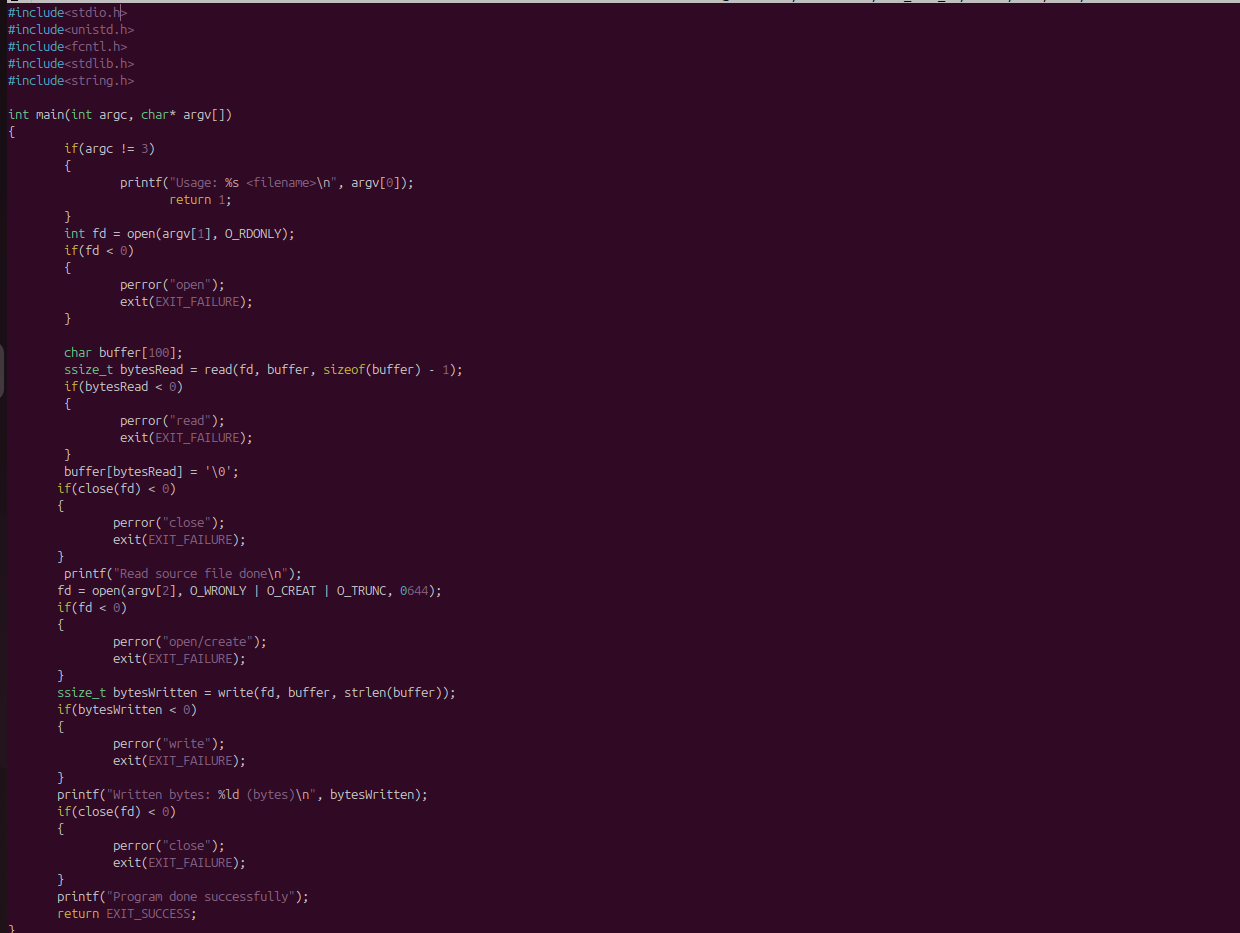
\includegraphics[width=1\linewidth]{figures/e3}
		\caption{Mã nguồn bài 3.}
		\label{fig:e3}
	\end{figure}
	
	Tương tự ở các bài trước, lần này em kiểm tra số lượng đối số truyền vào hàm main phải đủ 3 đối số bao gồm lệnh gọi chương trình, source file, destination file. \texttt{argv[]} sẽ lưu các đối số theo thứ tự được gọi lên trong lệnh chạy chương trình, tương ứng \texttt{argv[0]} sẽ là lệnh gọi chương trình, \texttt{argv[1]} sẽ lưu trữ tên source file và \texttt{argv[2]} sẽ lưu trữ tên destination file.
	
	Các thao tác còn lại giống hệt với bài ở trên.
	
	Kết quả khi chạy chuơng trình với 2 file là secondOutput.txt (ở bài 1) và e3\_resultt.txt (được tạo ra bằng hàm open thứ 2):
	\begin{figure}[H]
		\centering
		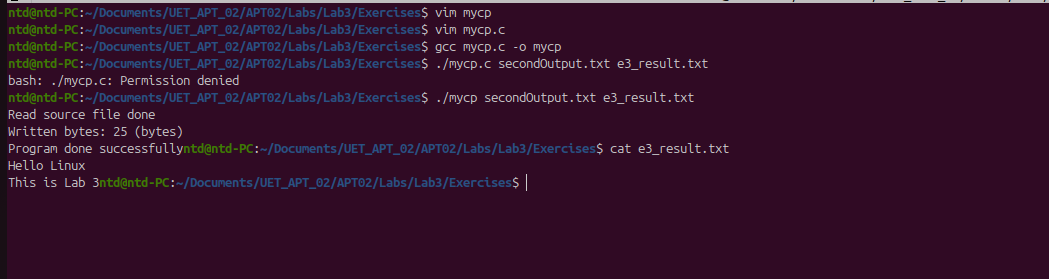
\includegraphics[width=0.7\linewidth]{figures/e3_result}
		\caption{Kết quả chạy chương trình với file secondOutput.txt và e3\_result.txt.}
		\label{fig:e3result}
	\end{figure}
	\section*{Bài 4}
	\begin{figure}[H]
		\centering
		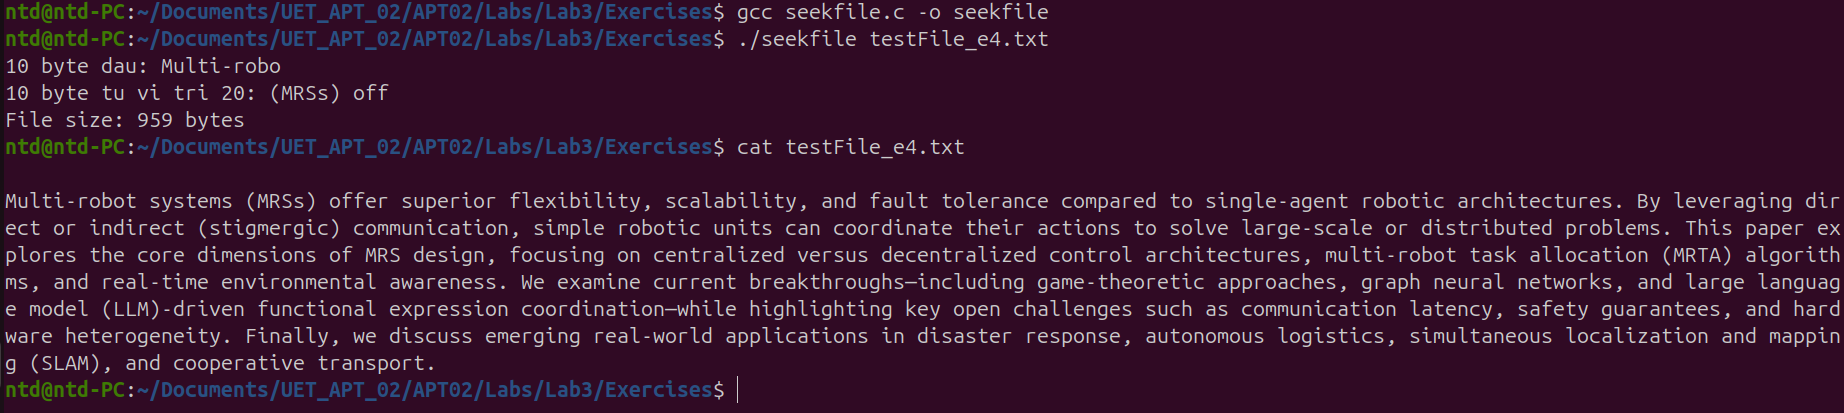
\includegraphics[width=1\linewidth]{figures/e4}
		\caption{Chương trình seekfile với file testFile\_e4.txt.}
		\label{fig:e4}
	\end{figure}
	
	\section*{Bài 5}
	\begin{figure}[H]
		\centering
		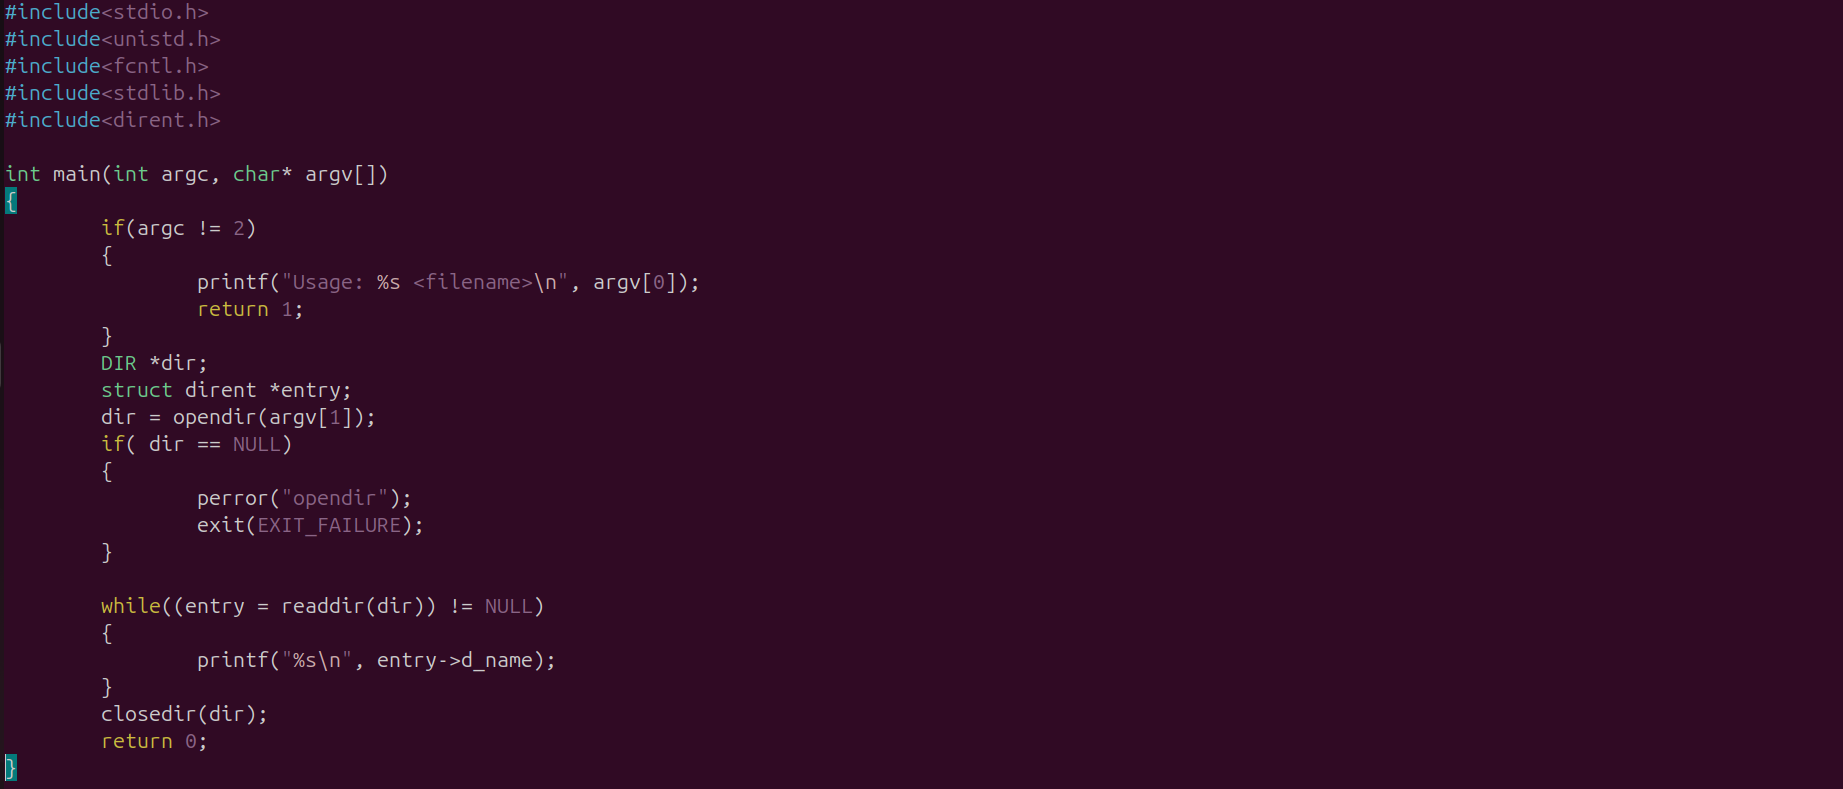
\includegraphics[width=1\linewidth]{figures/e5}
		\caption{Mã nguồn chương trình myls.}
		\label{fig:e5}
	\end{figure}
	
	Kết quả khi chạy thử chương trình:
	\begin{figure}[H]
		\centering
		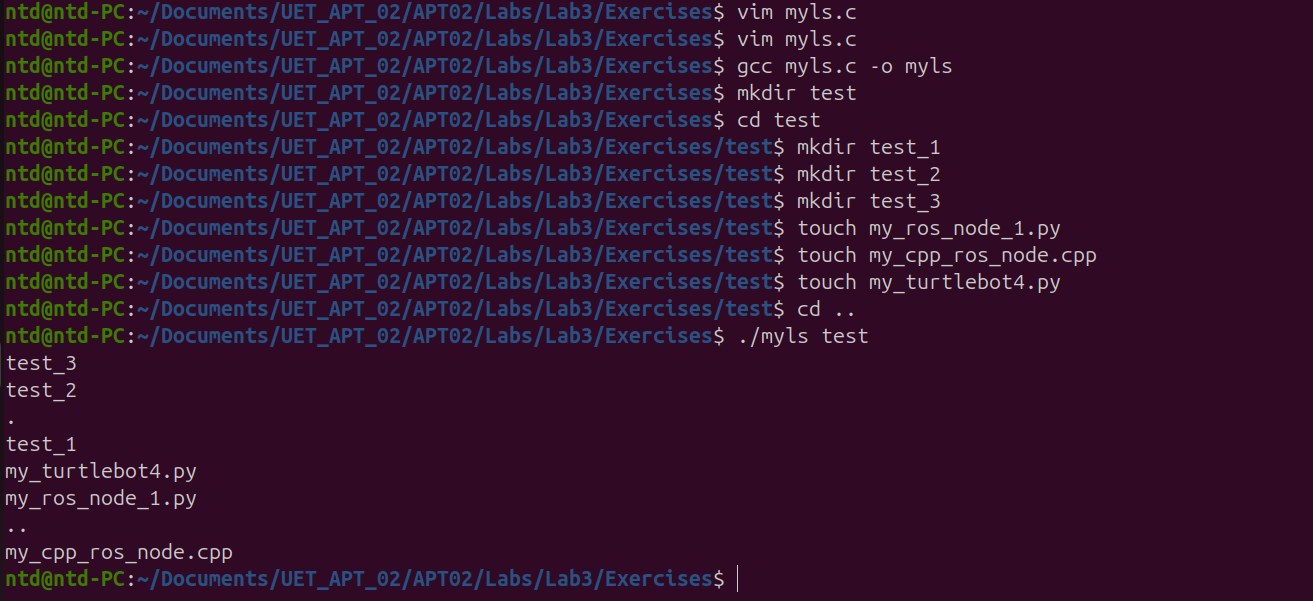
\includegraphics[width=1\linewidth]{figures/e5_result}
		\caption{kết quả chạy chương trình myls với thư mục test.}
		\label{fig:e5result}
	\end{figure}
\end{document}